\documentclass[a4paper]{article}

\usepackage[english]{babel}
\usepackage[utf8]{inputenc}
\usepackage{amsmath}
\usepackage{graphicx}
\usepackage[colorinlistoftodos]{todonotes}
\usepackage{caption}
\usepackage{subcaption}

\title{Computational Photography}

\author{Mich\`ele Wyss, 10-104-123}

\date{October 2, 2014}

\graphicspath{{imgs/}}
\begin{document}
\maketitle
\section*{The Spanish Castle illusion}
The Spanish Castle illusion is an astonishing effect to demonstrate how the human eye adapts to context in an image. 
Color perception is a relative thing that depends on the surrounding context. By constructing an ``inverted'' image, we can demonstrate how the human eye can be influenced... \todo{to be continued}
\section*{Example images}
\begin{figure}[ht]
	\centering
	\begin{subfigure}[h]{0.48\textwidth}
		\centering
		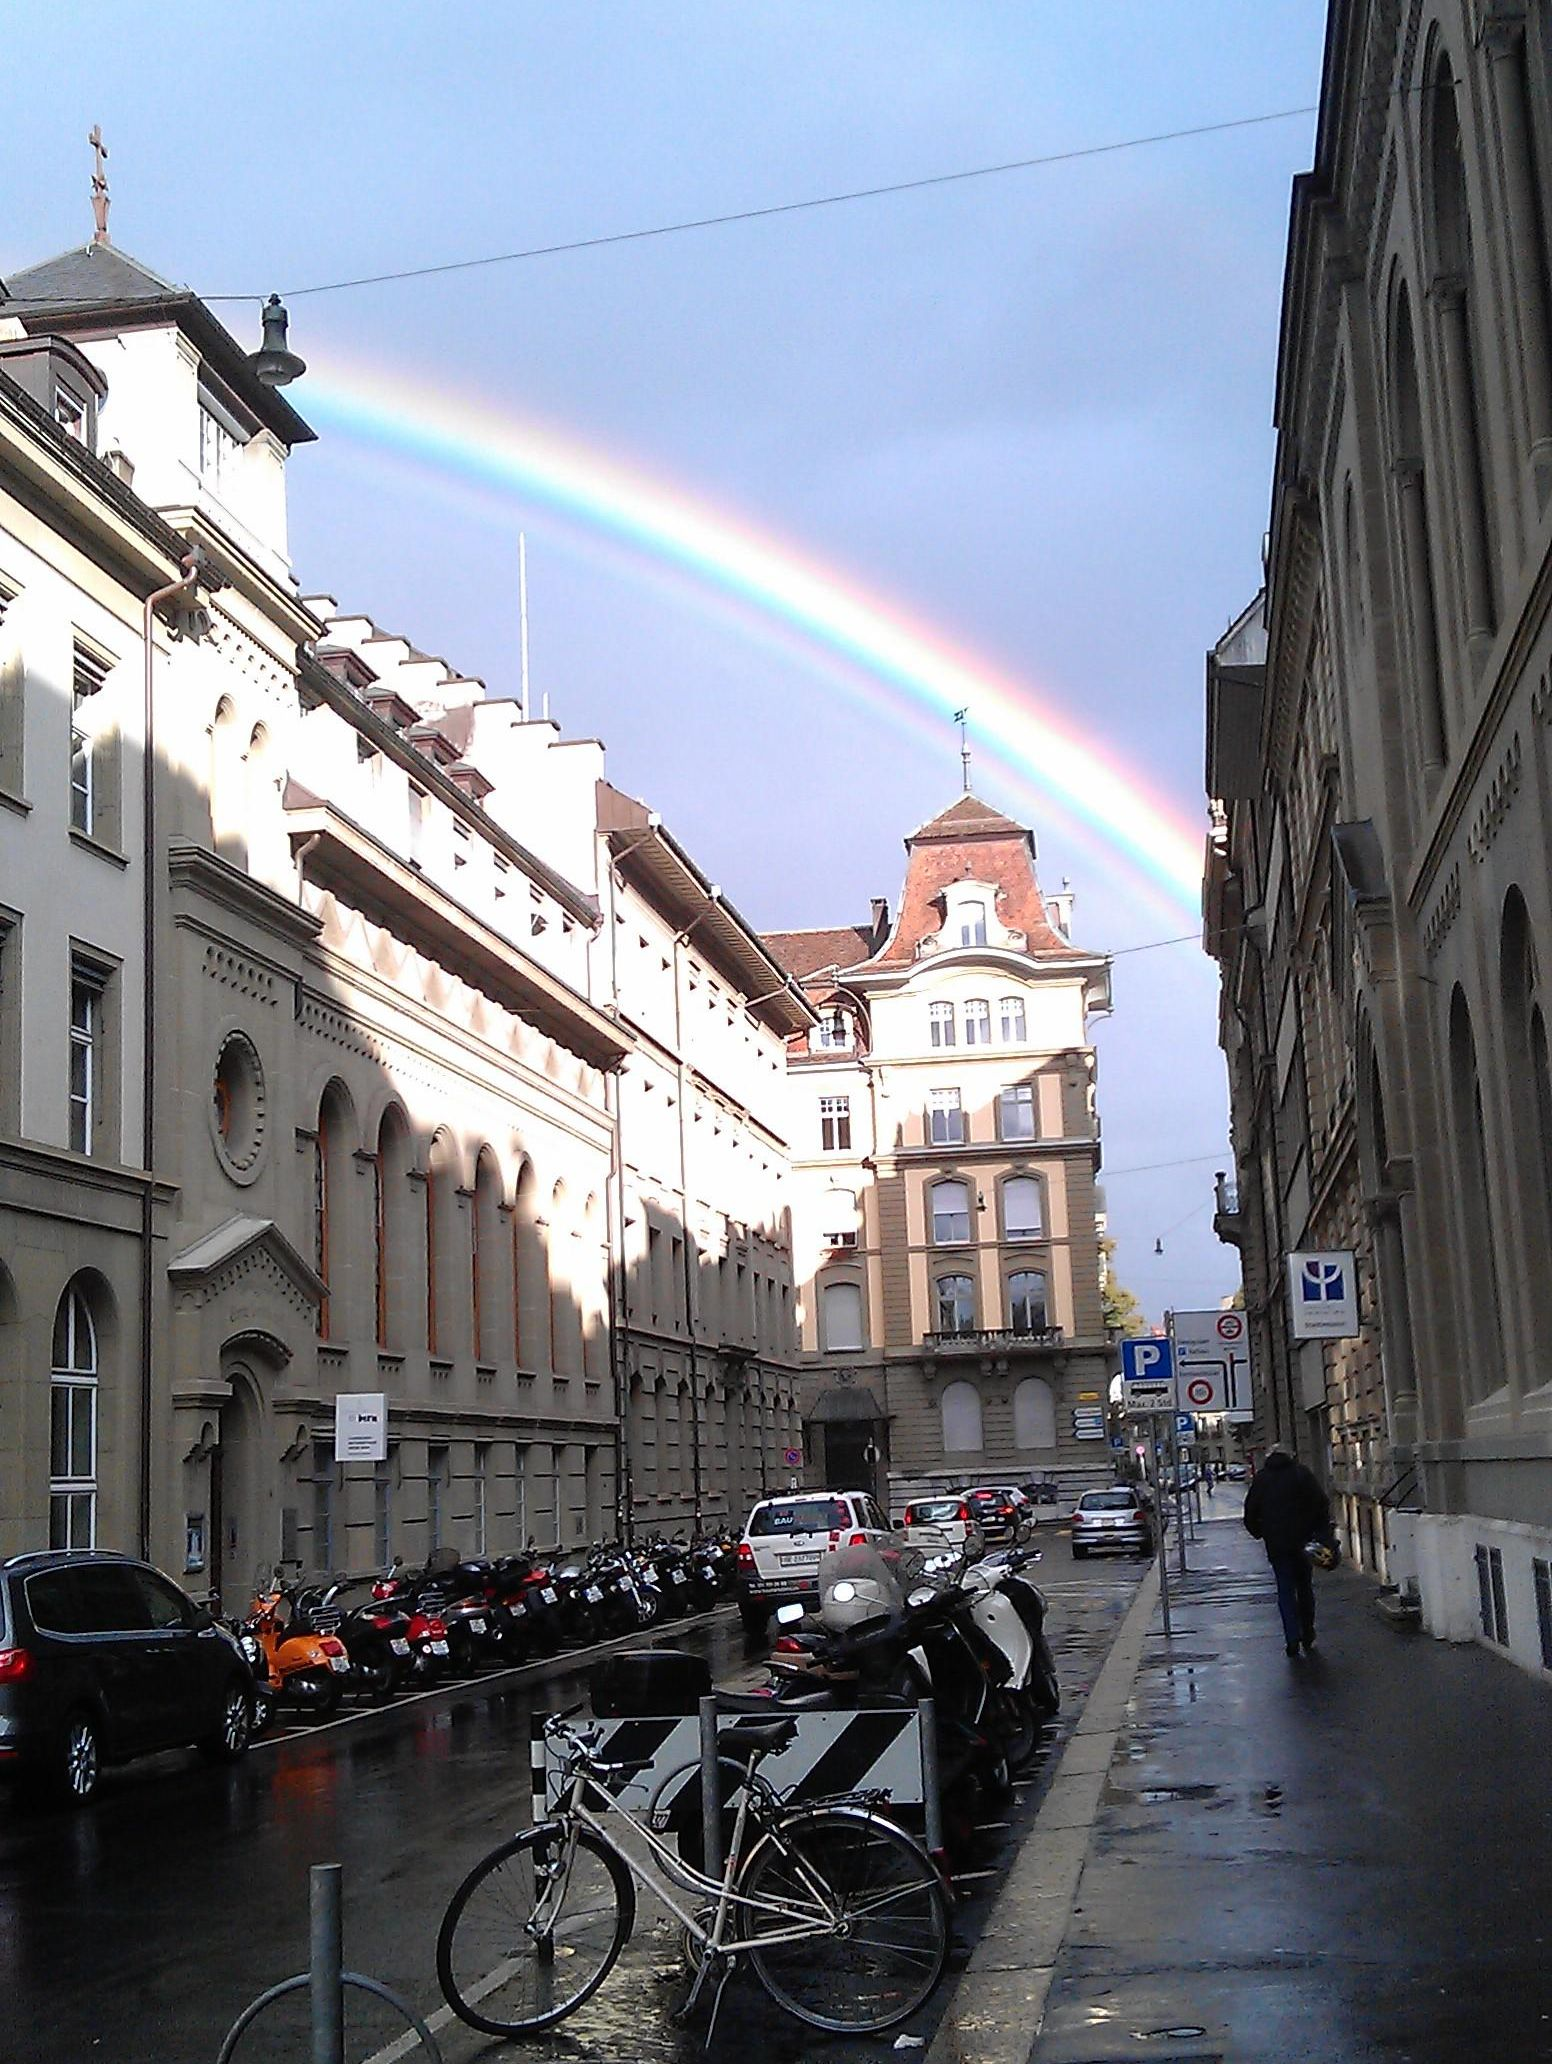
\includegraphics[width=\textwidth]{rainbow}
		\caption*{Input image}
	\end{subfigure}
	
	\vspace{3mm}
	\begin{subfigure}[h]{0.48\textwidth}
		\centering
		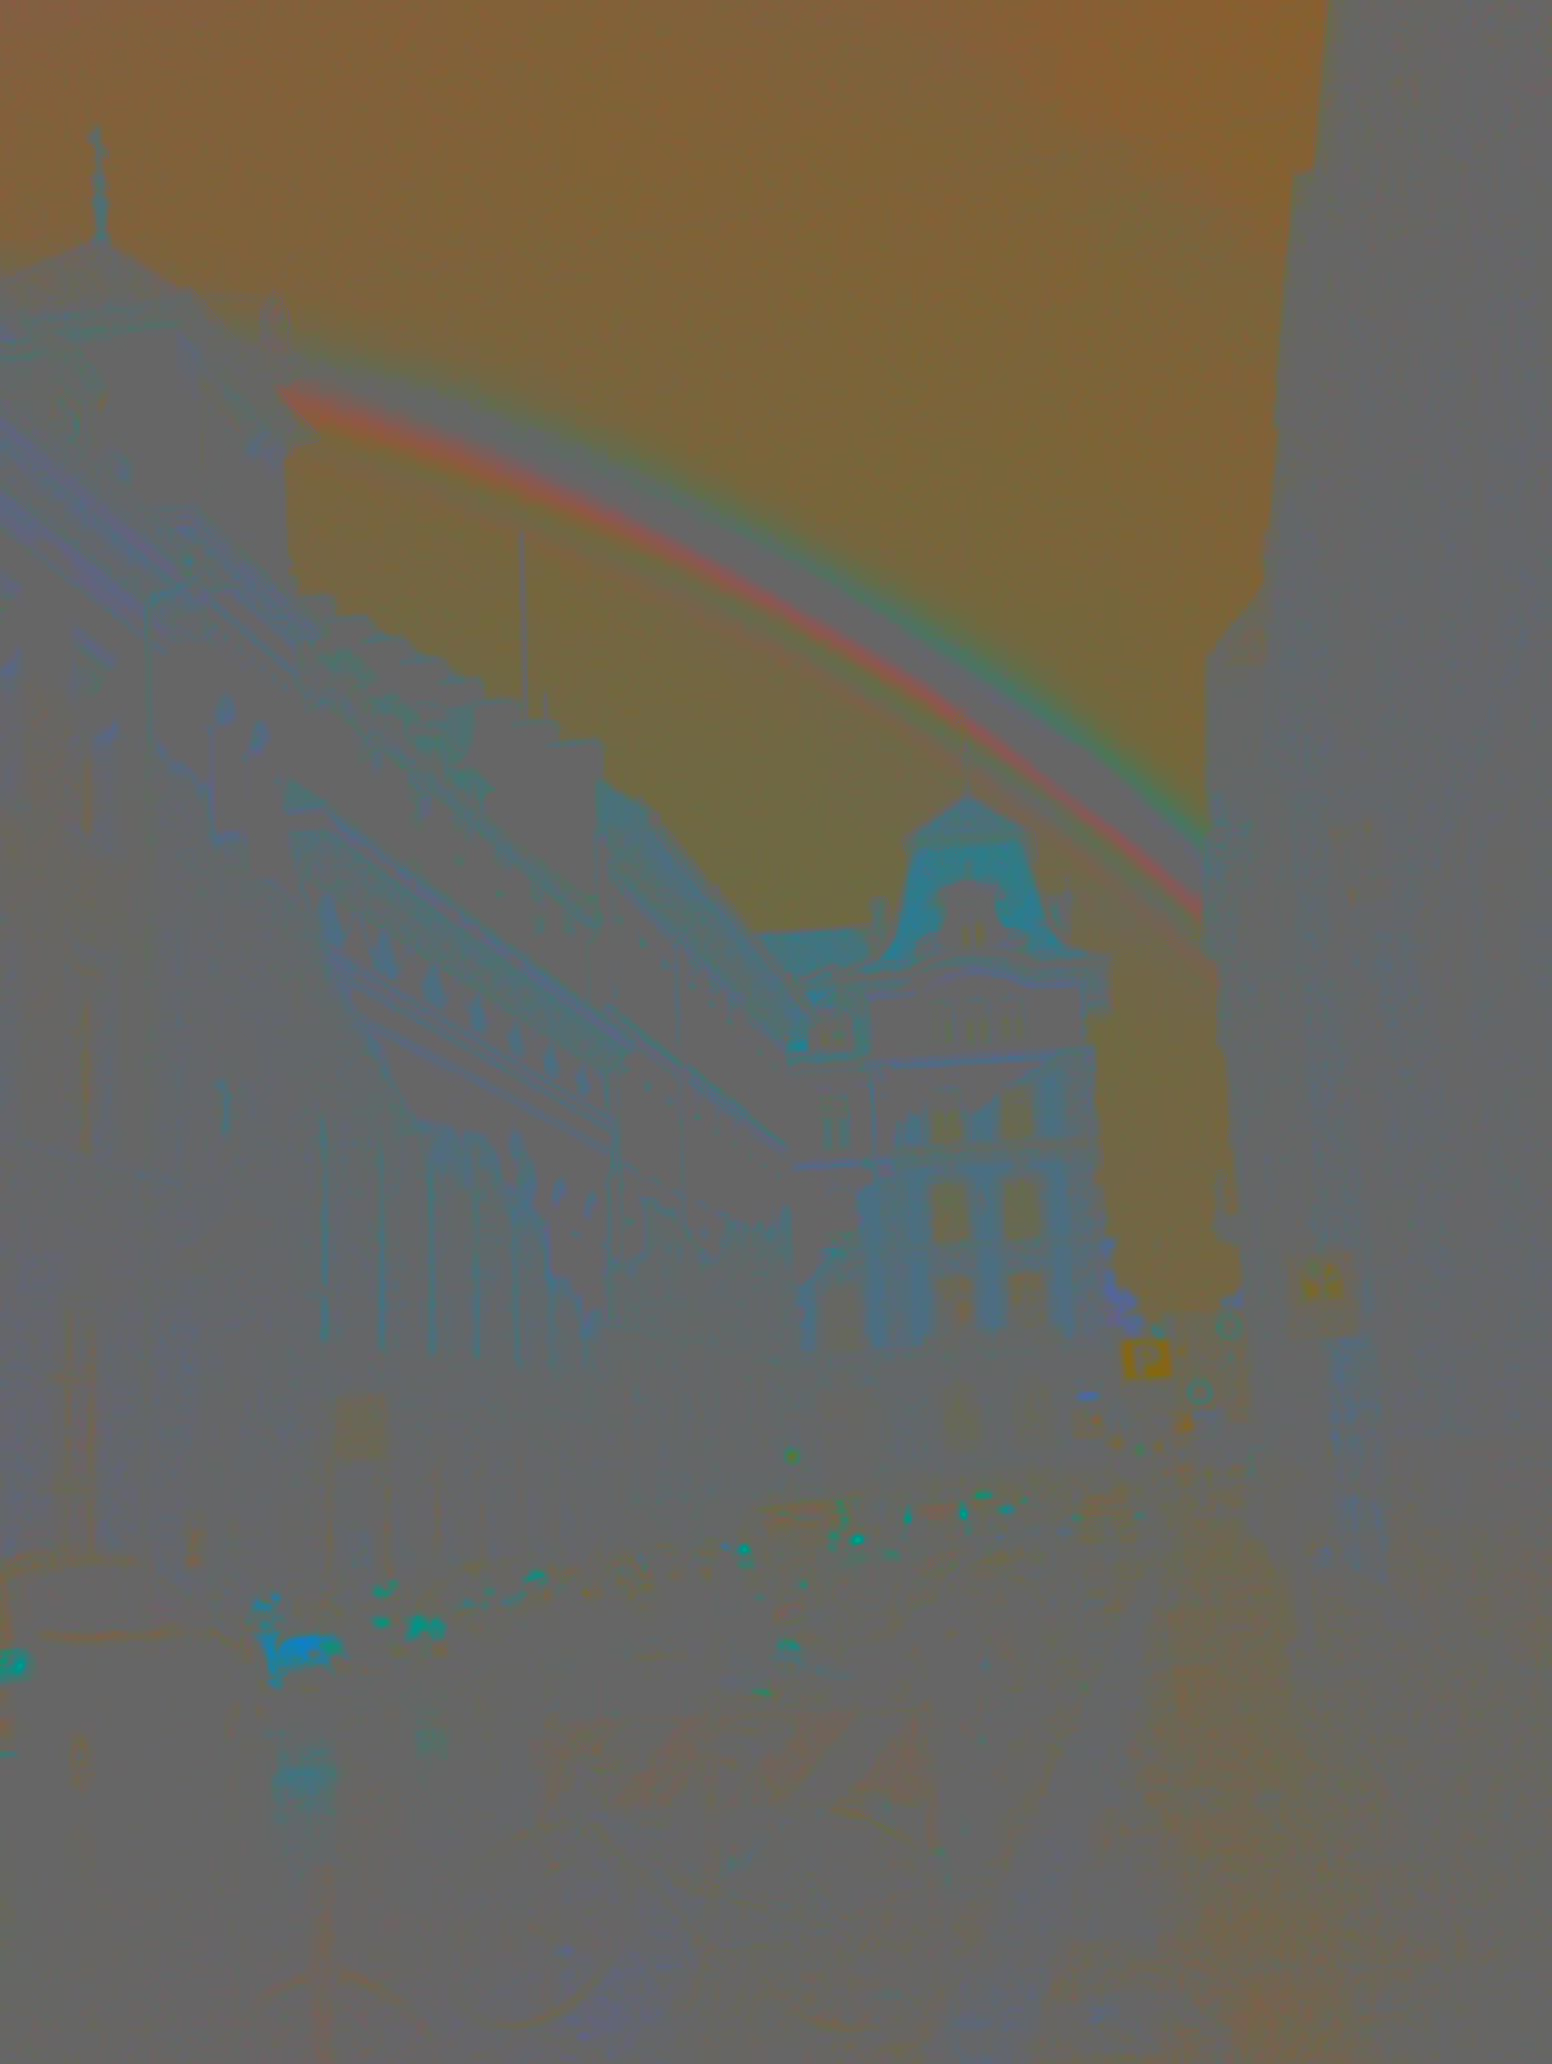
\includegraphics[width=\textwidth]{rainbow_inv}
		\caption*{Inverted image}
	\end{subfigure}
	~
	\begin{subfigure}[h]{0.48\textwidth}
		\centering
		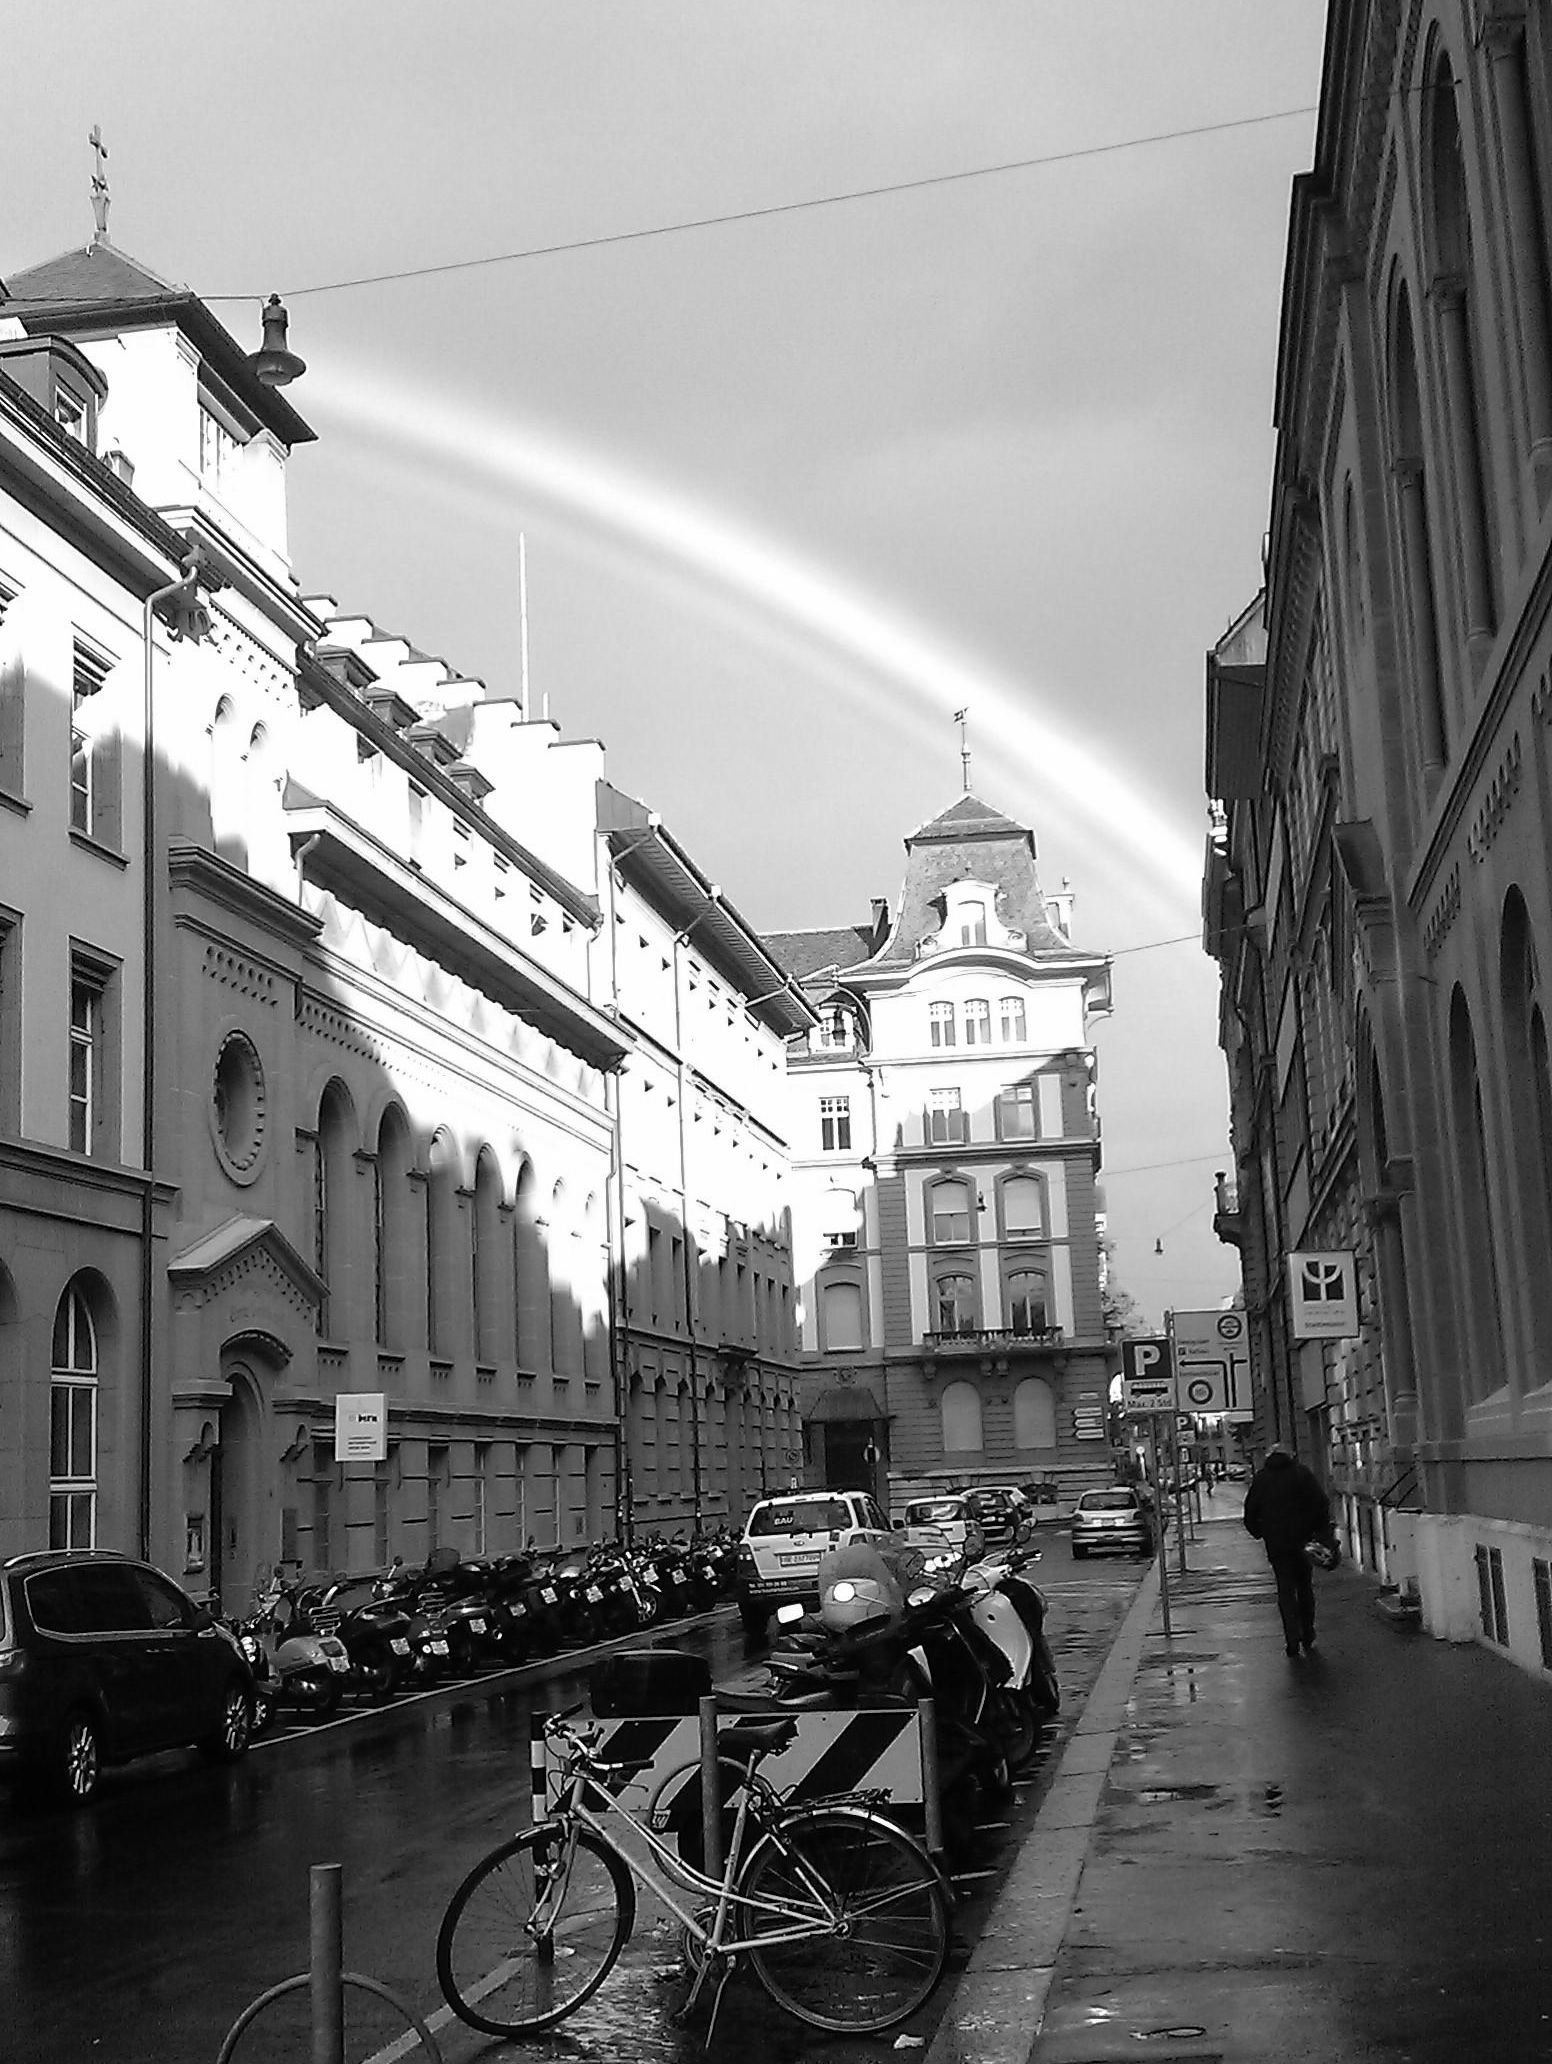
\includegraphics[width=\textwidth]{rainbow_gray}
		\caption*{Gray-scale image}
	\end{subfigure}	
\caption{The spanish castle illusion with the example of a photograph with a rainbow captured in Bern in September 2013.}
\label{fig:rainbow}
\end{figure}

\end{document}